\documentclass[preprint]{sigplanconf}

\usepackage{amssymb}
\usepackage{multicol}
\usepackage{xcolor}
\usepackage{graphicx}
\usepackage[fleqn]{amsmath}
\usepackage[hang,flushmargin]{footmisc} 
\usepackage{graphics} 
\usepackage{stmaryrd}
\usepackage{amsthm}
\usepackage[hyphens]{url}
\usepackage{hyperref}
\usepackage{ftnright}
\usepackage[notquote]{hanging}
\usepackage[T1]{fontenc}
\usepackage{semantic}

% =================================================================================================

% TODO: The model here does not actually use type erasure!!
% TODO: Maybe get rid of \mu_opt for records everywhere
% TODO: Disambigurate 's' as structural value and 's' as string
% TODO: Explain why we can only provide simple classes (!)
% TODO: Replace \nu_opt with \nu_? or something else that does not look shit

\urlstyle{sf}

\makeatletter
\renewcommand{\@makefntext}[1]{%
  \parindent 1em%
  \raggedright
  \begin{hangparas}{0.8em}{1}
  \noindent {$^{\@thefnmark}$~#1}
  \end{hangparas}
}
\makeatother

\newcommand{\langl}{\begin{picture}(4.5,7)
\put(1.1,2.5){\rotatebox{60}{\line(1,0){5.5}}}
\put(1.1,2.5){\rotatebox{300}{\line(1,0){5.5}}}
\end{picture}}
\newcommand{\rangl}{\begin{picture}(4.5,7)
\put(.9,2.5){\rotatebox{120}{\line(1,0){5.5}}}
\put(.9,2.5){\rotatebox{240}{\line(1,0){5.5}}}
\end{picture}}

\newcommand{\lang}{\begin{picture}(5,7)
\put(1.1,2.5){\rotatebox{45}{\line(1,0){6.0}}}
\put(1.1,2.5){\rotatebox{315}{\line(1,0){6.0}}}
\end{picture}}
\newcommand{\rang}{\begin{picture}(5,7)
\put(.1,2.5){\rotatebox{135}{\line(1,0){6.0}}}
\put(.1,2.5){\rotatebox{225}{\line(1,0){6.0}}}
\end{picture}} 

\newcommand{\llangl}{\langl\hspace{-0.35em}\langl}
\newcommand{\rrangl}{\rangl\hspace{-0.35em}\rangl}

\definecolor{cmtclr}{rgb}{0.0,0.6,0.0}
\definecolor{numclr}{rgb}{0.0,0.4,0.0}
\definecolor{kvdclr}{rgb}{0.0,0.0,0.6}
\definecolor{strclr}{rgb}{0.5,0.1,0.0}
\definecolor{prepclr}{rgb}{0.0,0.0,0.0}

\newcommand{\kvd}[1]{\textnormal{\textcolor{kvdclr}{\sffamily #1}}}
\newcommand{\num}[1]{\textnormal{\textcolor{numclr}{\sffamily #1}}}
\newcommand{\str}[1]{\textnormal{\textcolor{strclr}{\sffamily "#1"}}}
\newcommand{\strf}[1]{\textnormal{\textcolor{strclr}{\sffamily #1}}}
\newcommand{\ident}[1]{\textnormal{\sffamily #1}}
\newcommand{\lident}[1]{\textnormal{\sffamily\`{}\hspace{-0.25em}\`{}\hspace{-0.1em}#1\`{}\hspace{-0.25em}\`{}}}
\newcommand{\cmt}[1]{\textit{\sffamily\textcolor{cmtclr}{#1}}}

\newcommand{\lsep}[0]{\;\; | \;\;}
\newcommand{\narrow}[1]{\hspace{-0.85em} #1 \hspace{-0.85em}}

\newcommand{\tsep}[0]{\; \triangledown \;}
\newcommand{\tytag}{\ident{tag}}
\newcommand{\dropopt}[1]{\lfloor#1\rfloor}
\newcommand{\addopt}[1]{\lceil#1\rceil}
\newcommand{\tytagof}{\ident{tagof}}
\newcommand{\nameoftag}{\ident{nameof}}

\newcommand{\reduce}{\rightsquigarrow}

\newcommand{\sem}[1]{\llbracket #1 \rrbracket}
\newcommand{\semalt}[1]{\llangl #1 \rrangl}

\newtheorem{definition}{Definition}
\newtheorem{theorem}{Theorem}

% =================================================================================================

\begin{document}

\special{papersize=8.5in,11in}
\setlength{\pdfpageheight}{\paperheight}
\setlength{\pdfpagewidth}{\paperwidth}
\conferenceinfo{CONF 'yy}{Month d--d, 20yy, City, ST, Country} 
\copyrightyear{20yy} 
\copyrightdata{978-1-nnnn-nnnn-n/yy/mm} 
\doi{nnnnnnn.nnnnnnn}

%\titlebanner{banner above paper title}        % These are ignored unless
%\preprintfooter{short description of paper}   % 'preprint' option specified.

\title{F\# Data: \textnormal{Making structured data first-class citizens}}
%\subtitle{Subtitle Text, if any}

\authorinfo{Tomas Petricek}
           {University of Cambridge}
           {tomas@tomasp.net}
\authorinfo{Gustavo Guerra}
           {Microsoft Corporation, London}
           {gustavo@codebeside.org}
\authorinfo{Don Syme}
           {Microsoft Research, Cambridge}
           {dsyme@microsoft.com}
\maketitle

% =================================================================================================

\begin{abstract}
Most statically typed languages assume that programs run in a closed world, but this is not the 
case. Modern applications interact with external services and often access data in structured 
formats such as XML, CSV and JSON. Static type systems do not understand such external data sources
and only make data access more cumbersome. Should we just give up and leave the messy world of 
external data to dynamic typing and runtime checks?

Of course, we should not give up! In this paper, we show how to integrate external data sources 
into the F\# type system. As most real-world data on the web do not come with an explicit schema, 
we develop a type inference algorithm that infers a type from representative samples. Next, we use 
the type provider mechanism for integrating the inferred structures into the F\# type
system. 

The resulting library significantly reduces the amount of code that developers need to write when 
accessing data. It also provides additional safety guarantees. Arguably, as much as possible 
if we abandon the incorrect closed world assumption.
\end{abstract}

\category{D.3.3}{Programming Languages}{Language Constructs and Features }
\keywords F\#, Type Providers, JSON, XML, Data, Type Inference



% =================================================================================================
%
%   ###                                                                       
%    #  #    # ##### #####   ####  #####  #    #  ####  ##### #  ####  #    # 
%    #  ##   #   #   #    # #    # #    # #    # #    #   #   # #    # ##   # 
%    #  # #  #   #   #    # #    # #    # #    # #        #   # #    # # #  # 
%    #  #  # #   #   #####  #    # #    # #    # #        #   # #    # #  # # 
%    #  #   ##   #   #   #  #    # #    # #    # #    #   #   # #    # #   ## 
%   ### #    #   #   #    #  ####  #####   ####   ####    #   #  ####  #    # 
%
% =================================================================================================

\section{Introduction}
\label{sec:introduction}

The key function of many modern applications is to connect multiple data sources or services and
present the aggregated data in some form. Mobile applications for taking notes, searching train
schedules or finding tomorrow's weather all communicate with one or more services over the internet.

Increasing number of such services provide REST-based end-points that return data as CSV, XML
or JSON. Despite numerous schematization efforts, the services typically do not come with schema.
At best, the documentation provides a number of typical requests and sample responses.

For example, the OpenWeatherMap service provides an end-point for getting current weather for a 
given city\footnote{See ``Current weather data'': \url{http://openweathermap.org/current}}. The page documents the input 
URL parameters and shows one sample JSON response to illustrate the response structure.
Using a standard library for working with JSON and HTTP, we might call the service and 
read the temperature as follows \footnote{We abbreviate the full URL: 
\url{http://api.openweathermap.org/data/2.5/weather?q=Prague\&units=metric}}:

\noindent
\begin{equation*}
\begin{array}{l}
 \kvd{let}~\ident{data}=\ident{Http.Request}(\str{http://weather.org/?q=Prague}) \\[0.1em]
 \kvd{match}~\ident{JsonValue.Parse}(\ident{data})~\kvd{with} \\[0.1em]
 |~\ident{Record}(\ident{root})\rightarrow \\[0.1em]
 \quad \kvd{match}~\ident{Map.find}~\str{main}~\ident{root}~\kvd{with} \\[0.1em]
 \quad |~\ident{Record}(\ident{main})\rightarrow \\[0.1em]
 \quad \quad \kvd{match}~\ident{Map.find}~\str{temp}~\ident{main}~\kvd{with} \\[0.1em]
 \quad \quad |~\ident{Number}(\ident{num})\rightarrow \ident{printfn}~\str{Lovely \%f degrees!}~\ident{num} \\[0.1em]
 \quad \quad |~\_\rightarrow \ident{failwith}~\str{Incorrect format} \\[0.1em]
 \quad |~\_\rightarrow \ident{failwith}~\str{Incorrect format} \\[0.1em]
 |~\_\rightarrow \ident{failwith}~\str{Incorrect format} 
\end{array}
\end{equation*}
\vspace{0.1em}

\noindent
The code assumes that the response has a particular format described in the documentation. The
root node must be a record with a \str{main} field, which has to be another record containing
a \str{temp} field with numerical value. When the format is incorrect, the data access simply fails
with an exception.

Using the JSON type provider from the F\# Data library, we can write code with exactly the 
same functionality in two lines:

\vspace{-0.6em}
\begin{equation*}
\begin{array}{l}
 \kvd{type}~\ident{W} = \ident{JsonProvider}\langl\str{http://weather.org/?q=Prague}\rangl \\[0.1em]
 \ident{printfn}~\str{Lovely \%f degrees!}~(\ident{W.GetSample().Main.Temp})
\end{array}
\end{equation*}
\vspace{0.0em}

\noindent
On the first line, $\ident{JsonProvider}\langl\str{...}\rangl$ invokes a type provider at 
compile-time with the URL as a sample. The type provider infers the structure of the response
and provides a type with a \ident{GetSample} method that returns a parsed JSON with nested
properties \ident{Main.Temp}, returning the temperature as a number.

In the rest of the paper, we give more detailed description of the mechanism and we also discuss
theoretical safety properties of the approach. The key novel contributions of this paper are:

\begin{itemize}
\item We present type providers for XML, CSV and JSON (Section~\ref{sec:providers}) 
  that are available in the F\# Data library and we also cover practical aspects of the 
  implementation that contributed to their industrial adoption (Section~\ref{sec:impl}). 

\item We describe a predictable type inference algorithm for structured data formats that
  underlies the type providers (Section~\ref{sec:inference}). It is based on finding common 
  supertype of a set of examples.

\item We provide a minimal formal model (Section~\ref{sec:formal}) and use it to prove a
  relativized notion of type safety for our type providers (Section~\ref{sec:safety}). Although 
  we focus on our specific case, the relativized safety property demonstrates a new way of 
  thinking about ML-style type safety that is needed in the context of web.
\end{itemize}

\noindent
Although the F\# Data library has been widely adopted is one of the most downloaded F\# libraries 
it has not yet been presented in an academic form. Additional documentation and source code can 
be found at \url{http://fsharp.github.io/FSharp.Data}.



% =================================================================================================
%
%   #######                                                                                  
%      #    #   # #####  ######    #####  #####   ####  #    # # #####  ###### #####   ####  
%      #     # #  #    # #         #    # #    # #    # #    # # #    # #      #    # #      
%      #      #   #    # #####     #    # #    # #    # #    # # #    # #####  #    #  ####  
%      #      #   #####  #         #####  #####  #    # #    # # #    # #      #####       # 
%      #      #   #      #         #      #   #  #    #  #  #  # #    # #      #   #  #    # 
%      #      #   #      ######    #      #    #  ####    ##   # #####  ###### #    #  ####  
%
% =================================================================================================

\section{Structural type providers}
\label{sec:providers}

We start with an informal overview that shows how F\# Data type providers simplify working with 
JSON, XML and CSV. We also introduce the necessary aspects of F\# 3.0 type providers along the 
way. The examples in this section illustrate a number of key properties of our type inference 
algorithm:

\begin{itemize}
\item Our mechanism is robust and predictable. This is important as the user directly works with 
  the inferred types and should understand why a specific type was inferred from a given 
  sample\footnote{In particular, we do not use probabilistic methods where adding additional 
  sample could change the shape of the type.}.

\item Our inference mechanism prefers records over unions. This better supports developer tooling --
  most F\# editors provide code completion hints on ``.'' and so types with properties (records)
  are easier to use than types that require pattern matching.

\item Finally, we handle a number of practical concerns that may appear overly complicated, but
  are important in the real world. This includes support for different numerical types, \kvd{null}
  values and missing data and also different ways of representing Booleans in CSV files.
\end{itemize}

% --------------------------------------------------------------------------------------------------

\subsection{Working with JSON documents}
\label{sec:providers-json}

The JSON format used in the example in Section~\ref{sec:introduction} is a popular format for data
exchange on the web based on data structures used in JavaScript. The following is the definition 
of the \ident{JsonValue} type used earlier to represent parsed JSON:
%
\begin{equation*}
\begin{array}{l}
 \kvd{type}~\ident{JsonValue} = \\[0.1em]
 \quad|~\ident{Null} \\[0.1em]
 \quad|~\ident{Number}~\kvd{of}~\ident{decimal} \\[0.1em]
 \quad|~\ident{String}~\kvd{of}~\ident{string} \\[0.1em]
 \quad|~\ident{Boolean}~\kvd{of}~\ident{bool} \\[0.1em]
 \quad|~\ident{Record}~\kvd{of}~\ident{Map}\langl\ident{string}, \ident{JsonValue}\rangl \\[0.1em]
 \quad|~\ident{Array}~\kvd{of}~\ident{JsonValue}[] \\[0.1em]
\end{array}
\end{equation*}
%
The OpenWeatherMap example in the introduction used only a (nested) record containing a numerical
value. To demonstrate other aspects of the JSON type provider, we look at a more complex example
that also involves \kvd{null} value and an array:
%
{\small{
\begin{verbatim}
  [ { "name": null, "age": 25 },
    { "name": "Alexander", "age": 3.5 },
    { "name": "Tomas" } ]
\end{verbatim}
}}
%
\noindent
Say we want to print the names of people in the list with an age if it is available. As before, 
the standard approach would be to pattern match on the parsed \ident{JsonValue}. The code would 
check that the top-level node is a \ident{Array}, iterate over the elements checking that each is
a \ident{Record} with certain properties and throw an exception or skip values in incorrect format.
The standard approach can be made nicer by defining helper functions. However, we still need to
specify names of fields as strings, which is error prone and can not be statically checked.

Assuming the \strf{people.json} file contains the above example and \ident{data} is a string value
that contains another data set in the same format, we can print names and ages as follows:
%
\begin{equation*}
\begin{array}{l}
 \kvd{type}~\ident{People}~=~\ident{JsonProvider}\langl\str{people.json}\rangl\hspace{1em} \\[0.6em]
 \kvd{let}~\ident{items}~=~\ident{People.Parse}(\ident{data})\\[0.1em]
 \kvd{for}~\ident{item}~\kvd{in}~\ident{items}~\kvd{do}\\[0.1em]
 \quad\ident{printf}~\str{\%s }~\ident{item.Name}\\[0.1em]
 \quad\ident{Option.iter}~(\ident{printf}~\str{(\%f)})~\ident{item.Age}
\end{array}
\end{equation*}
%
The code achieves the same simplicity as when using dynamically typed languages, but is statically 
type-checked. In contrast to the earlier example, we now use a local file \strf{people.json} as a 
sample for the type inference, but then processes data from another source. 

\paragraph{Type providers.}
The notation $\ident{JsonProvider}\langl\str{people.json}\rangl$ on the first line passes a 
\emph{static parameter} to the type provider. Static parameters are resolved at compile-time, 
so the file name has to be a constant. The provider analyzes the sample and generates
a type that we name \ident{People}. In F\# editors that use the F\# Compiler Service [?], the 
type provider is also executed at development-time and so the same provided types are
used in code completion.

The \ident{JsonProvider} uses a type inference algorithm (Section~\ref{sec:inference})  and
infers the following types from the sample:
%
\begin{equation*}
\begin{array}{l}
 \kvd{type}~\ident{Entity}~=  \\[0.1em]
 \quad \kvd{member}~\ident{Age}~:~\ident{option}\langl \ident{decimal}\rangl \\[0.1em]
 \quad \kvd{member}~\ident{Name}~:~\ident{option}\langl \ident{string}\rangl \\[0.6em]
 \kvd{type}~\ident{People}~=  \\[0.1em]
 \quad \kvd{member}~\ident{GetSample}~:~\ident{unit}~\rightarrow~\ident{Entity}[] \\[0.1em]
 \quad \kvd{member}~\ident{Parse}~:~\ident{string}~\rightarrow~\ident{Entity}[] \\[0.1em]
\end{array}
\end{equation*}
%
The type \ident{Entity} represents the person. The property \ident{Name} is optional, because
one of the sample records contains \kvd{null} as the name. The property \ident{Age} is also optional,
because the value is missing in one sample. The two sample ages are an integer \num{25} and a 
decimal \num{3.5} and so the common inferred type is \ident{decimal}.

The type \ident{People} provides two methods for reading data. \ident{GetSample} returns the
sample used for the inference and \ident{Parse} parses a JSON string containing data in the same 
format as the sample. Since the sample JSON is a collection of records, both methods return an 
array of \ident{Entity} values.

\paragraph{Error handling.}
In addition to the structure of the types, the type provider also specifies what code should be 
executed at run-time in place of \ident{item.Name} and other operations. This is done through a 
\emph{type erasure} mechanism demonstrated in Section~\ref{sec:providers-csv}. In this example,
the runtime behaviour is the same as in the hand-written sample in Section~\ref{sec:introduction} --
a member access throws an exception if the document does not have the expected format.

Informally, the safety property discussed in Section~\ref{sec:safety} states that if the inputs
are subtypes of some of the provided samples (\emph{i.e.}~the samples are representative), then
no exceptions will occur. In other words, we cannot avoid all failures, but we can prevent some --
for example, if the OpenWeatherMap changes the response format, the sample in Section~\ref{sec:introduction}
will not re-compile and the user knows that the code needs to be changed. What this means for
the traditional ML type safety is discussed in Section~\ref{sec:safety-discuss}.

\paragraph{The role of records.}
The sample code is easy to write thanks to the fact that most F\# editors provide code completion
when ``.'' is typed. The developer does not need to look at the sample JSON file to see what fields
are available for a person. To support this scenario, our inference algorithm prefers records
(we also treat XML elements and CSV rows as records).

In the above example, this is demonstrated by the fact that \ident{Age} is marked as optional.
An alternative is to provide two different record types (one with \ident{Name} and other with 
\ident{Name} and \ident{Age}), but this would complicate the processing code.

% --------------------------------------------------------------------------------------------------

\subsection{Reading CSV files}
\label{sec:providers-csv}

In the CSV file format, the structure is a collection of rows (records) consisting of fields 
(with names specified by the first row). The inference needs to infer the types of fields.
For example:
%
{\small{
\begin{verbatim}
  Ozone, Temp, Date,       Autofilled
  41,    67,   2012-05-01, 0
  36.3,  72,   2012-05-02, 1
  12.1,  74,   3 kveten,   0
  17.5,  #N/A, 2012-05-04, 0
\end{verbatim}
}}
%
\noindent
One difference between JSON and CSV formats is that in CSV, the literals have no data types.
In JSON, strings are \str{quoted} and Booleans are \kvd{true} and \kvd{false}. This is not the
case for CSV and so we need to infer not just the structure, but also the primitive types.

Assuming the sample is saved as \strf{airdata.csv}, the following snippet prints all
rows from another file that were not autofilled:
%
\begin{equation*}
\begin{array}{l}
 \kvd{type}~\ident{AirCsv}~=~\ident{CsvProvider}\langl\str{airdata.csv}\rangl\hspace{1em} \\[0.6em]
 \kvd{let}~\ident{air}~=~\ident{AirCsv.Parse}(\ident{data})\\[0.1em]
 \kvd{for}~\ident{row}~\kvd{in}~\ident{air.Rows}~\kvd{do}\\[0.1em]
 \quad\kvd{if}~\ident{not}~\ident{row.Autofilled}~\kvd{then}\\[0.1em]
 \quad\quad \ident{printf}~\str{\%s: \%d}~\ident{row.Date row.Ozone}\\
\end{array}
\end{equation*}
%
The type of the record (\ident{row}) is, again, inferred from the sample. The \ident{Date} column
uses mixed formats and is inferred as \ident{string} (although we support many date formats and 
``May 3'' would work). More interestingly, we also infer \ident{Autofilled} as Boolean, because 
the sample contains only $0$ and $1$ values and using those for Booleans is a common CSV convention.
Finally, the fields \ident{Ozone} and \ident{Temp} have types \ident{decimal} and
$\ident{option}\langl\ident{int}\rangl$.

\paragraph{Erasing type providers.}
At runtime, the type providers we describe use an erasure mechanism similar to Java Generics [?]. 
A type provider also generates code that is executed in place of the members of the generated types.
In the above example, the compiled (and actually executed) code looks as follows:
%
\begin{equation*}
\begin{array}{l}
 \kvd{let}~\ident{air}~=~\ident{CsvFile}\ident{.Load}(\str{airdata.csv}, \kvd{fun}~\ident{r}\rightarrow\\[0.1em]
 \quad \ident{asDecimal r}.[\num{0}], \ident{asIntOpt r}.[\num{1}], \ident{r}.[\num{2}], \ident{asBool r}.[\num{3}])\\[0.6em]
 \kvd{for}~\ident{c1},\_,\ident{c3},\ident{c4} ~\kvd{in}~\ident{air.Rows}~\kvd{do}\\[0.1em]
 \quad\kvd{if}~\ident{not}~\ident{c4}~\kvd{then}~\ident{printf}~\str{\%s: \%d}~\ident{c3 c1}\\
\end{array}
\end{equation*}
%
The generated type \ident{AirCsv} is erased to a type $\ident{CsvFile}\langl\alpha\rangl$.
The \ident{Load} method takes the file name together with a function that turns a row represented 
as an array of strings to a typed representation -- here, a four-element tuple 
$\ident{decimal}*\ident{option}\langl\ident{int}\rangl*\ident{string}*\ident{bool}$ (this type
is also used as a type argument of $\ident{CsvFile}\langl\alpha\rangl$. The properties
such as \ident{Ozone} are then replaced with an accessor that reads the corresponding tuple
element.

The type erasure mechanism is explained in our simplified formal model in Section~\ref{sec:formal}.
More details about the full implementation in F\# can be found in the paper on F\# type 
providers [?].

% -------------------------------------------------------------------------------------------------

\subsection{Processing XML data}
\label{sec:providers-xml}

The XML format is similar to JSON in that it uses nested elements rather than a flat CSV-like 
structure. In our inference algorithm, we use the notion of \emph{records} for both JSON records 
and XML elements. However, unlike in JSON, the XML elements also have a name. An element can 
contain a collection of child elements. In case of XML, the collection can often be heterogeneous 
containing child nodes of different names. Consider the following (simplified) RSS news feed as an example:
%
{\small{
\begin{verbatim}
  <rss version="2.0"><channel>
    <title> BBC News - Europe </title>
    <item><title> Kurdish activists 
        killed in Paris </title></item>
    <item><title> German MPs warn 
        over UK EU exit </title></item>
  </channel></rss>
\end{verbatim}
}}
%
\noindent
The \ident{channel} node contains a single \ident{title} node (with the name of the feed) and multiple 
\ident{item} nodes (individual news articles). In RSS, the \ident{title} nodes always contain plain text,
while \ident{item} nodes contain \ident{title} (and also \ident{url} and othe properties omitted here).

When extracting data from such XML documents, we often need to get nodes of a specific name (all
items) or extract the content of a node (feed title). The XML type provider is optimized for 
this style of access and allows processing the feed as follows:

\noindent
\begin{equation*}
\begin{array}{l}
 \kvd{type}~\ident{RssFeed}~=~\ident{XmlProvider}\langl\str{rss-sample.xml}\rangl\hspace{1em} \\[0.5em]
 \kvd{let}~\ident{channel}~=~\ident{RssFeed.Load}(\str{http://bbc.co.uk/...}).\ident{Channel}\\
 \ident{printf}~\str{News from: \%s }~\ident{channel.Title}\\
 \kvd{for}~\ident{item}~\kvd{in}~\ident{channel.Items}~\kvd{do}\\
 \quad\ident{printf}~\str{ - \%s }~\ident{item.Title}\\
\end{array}
\end{equation*}
%
In this example, the type of the \ident{channel} value represents a heterogeneous collection
that contains exactly one \ident{title} node and zero or more \ident{item} nodes.

\paragraph{Heterogeneous collections and unions.}
Our inference algorithms recognizes this as a \emph{heterogeneous collection} (if the same structure 
appears in all samples) and generates a type with a member \ident{Title} for accessing the value 
of the singleton \ident{title} element together with a member \ident{Items} that returns a 
collection of zero or more items. As a further simplification, if an element contains only a 
primitive value (such as \ident{title}) it is represented as a value of primitive type (so 
\ident{channel.Title} has a type \ident{string}).

As an alternative, the inference could produce a collection of union type (with a case for \ident{item}
and a case for \ident{title}). This alternative is useful for documents with complicated structure 
(such as XHTML files), but less useful for files with simpler structure such as web server responses,
data stores and configuration files. 

Moreover, our approach based on heterogeneous collections has a nice property that it generates types
with the same public interface for the following two ways of representing data in XML:
%
{\small{
\begin{verbatim}
  <author name="Tomas" age="27" />
  <author><name>Tomas</name><age>27</age></author>
\end{verbatim}
}}
%
\noindent
In both cases, the provided type for \ident{author} has two properties, typed \ident{string} and 
\ident{int} respectively. In Section~\ref{sec:inference}, we discuss the simplified model (using 
union types). The inference based on heterogeneous collections is described later in 
Section~\ref{sec:impl-collections}.

% -------------------------------------------------------------------------------------------------

\subsection{Summary}
The previous three sections demonstrated the F\# Data type providers for JSON, CSV and XML.
A reader interested in more examples is invited to look at documentation on the F\# Data web 
site\footnote{Available at \url{http://fsharp.github.io/FSharp.Data/}}.

It should be noted that we did not attempt to present the library using well-structured ideal 
samples, but instead used data sets that demonstrate typical issues that are frequent in real 
world inputs (missing data, inconsistent encoding of Booleans and heterogeneous structures).

From looking at just the previous three examples, these may appear arbitrary, but our experience
suggests that they are the most common issues. The following JSON response with government debt
information returned by the World Bank API [?] demonstrates all three problems:
%
{\small{
\begin{verbatim}
  [ { "page": 1, "pages": 5 },
    [ { "indicator": "GC.DOD.TOTL.GD.ZS",
        "date": "2012",
        "value": null },
      { "indicator": "GC.DOD.TOTL.GD.ZS",
        "date": "2010",
        "value": "35.1422970266502" } ] ]
\end{verbatim}
}}
%
\noindent
First of all, the top-level element is a collection containing two values of different kind.
The first is a record with meta-data about the current page and the second is an array with data. 
The JSON type provider infers this as heterogeneous collection with properties \ident{Record}
for the former and \ident{Array} for the latter. Second, the \ident{value} is \kvd{null} for some
records. Third, numbers can be represented in JSON as numeric literals (without quotes), but
here, they are returned as string literals instead\footnote{This is often used to avoid non-standard
numerical types in JavaScript.}.


% =================================================================================================
%
%   #######                                                                                  
%      #    #   # #####  ######    # #    # ###### ###### #####  ###### #    #  ####  ###### 
%      #     # #  #    # #         # ##   # #      #      #    # #      ##   # #    # #      
%      #      #   #    # #####     # # #  # #####  #####  #    # #####  # #  # #      #####  
%      #      #   #####  #         # #  # # #      #      #####  #      #  # # #      #      
%      #      #   #      #         # #   ## #      #      #   #  #      #   ## #    # #      
%      #      #   #      ######    # #    # #      ###### #    # ###### #    #  ####  ###### 
%
% =================================================================================================

\section{Structural type inference}
\label{sec:inference}

Our type inference algorithm for structured formats is based on a subtyping relation. When 
inferring the type of a document, we infer the most specific types of individual values (CSV rows,
JSON or XML nodes) and find a common supertype of values in the sample.

In this section, we define the \emph{structural type} $\sigma$, which is a type of structured data.
Note that this type is distinct from the programming language types $\tau$ (the type generates the
latter from the former). Next, we define the subtyping relation on structural types $\sigma$ and 
describe the algorithm for finding a common supertype. 

Note that the subtyping relation between structural types $\sigma$ does not map to a subtyping 
relation between F\#  types $\tau$. However, it does hold at runtime, meaning that an operation on 
a supertype can be performed on its subtypes. We make the type provider mechanism and runtime aspects 
precise in Section~\ref{sec:formal} before discussing safety in Section~\ref{sec:safety}.

\subsection{Structural types}
\label{sec:inference-types}

The grammar below defines \emph{structural type} $\sigma$. We distinguish between \emph{non-nullale types}
that always have a valid value (written as $\hat{\sigma}$) and \emph{nullable types} that encompass missing 
and \kvd{null} values (written as $\sigma$). We write $\nu$ for record field names and $\nu_{\ident{opt}}$
for record names, which can be empty:
%
\begin{equation*}
\begin{array}{rcl}
 \hat{\sigma} &\narrow{=}& \nu_{\ident{opt}}\; \{ \nu_1 : \sigma_1, \ldots, \nu_n : \sigma_n \} \\[0.1em]
                &\narrow{|}& \ident{float} \lsep \ident{decimal} \lsep \ident{int} \lsep \ident{bit} \lsep \ident{bool} \lsep \ident{string} 
 \\[0.6em] 
       \sigma &\narrow{=}& ~\hat{\sigma}~ \lsep \hat{\sigma}\;\,\kvd{option} \lsep [\sigma] \\[0.1em]
              &\narrow{|}& \sigma_1 + \ldots + \sigma_n \lsep ~\top~ \lsep \kvd{null}
\end{array}
\end{equation*}
%
The non-nullable types include records (consisting of an optional name and zero or more fields with
their types) and primitive types. Records arising from XML documents are always named, while records
used by JSON and CSV providers are always unnamed. 

Next, we have three numerical types -- \ident{int} for integers, \ident{decimal} for small high-precision 
decimal numbers and \ident{float} for floating-point numbers (these are related by sub-typing relation as
discussed in the next section). Furthermore, the \ident{bit} type is a type of values $0$ and $1$ and 
makes it possible to infer Boolean in the CSV processing example discussed in Section~\ref{sec:providers-csv}.

Any non-nullable type is also a nullable type, but it can be wrapped in the \kvd{option}
constructor to explicitly permit the \kvd{null} value. These are typically mapped to the standard F\# option 
type. A simple collection type $[\sigma]$ is also nullable and missing values or \kvd{null} are treated as 
empty collection. The type $\kvd{null}$ is inhabited by the $\kvd{null}$ value (using an overloaded but not
ambiguous notation) and $\top$ represents the top type.

Finally, a union type in our model implicitly permits the \kvd{null} value. This is because structural union 
types are \emph{not} mapped to F\# union types. Instead our encoding requires the user to handle the 
cases one-by-one and so they also need to handle the situation when none of the cases matches (as discussed
in Section~\ref{sec:impl-unions}, this is the right choice for an F\# type provider, but it would not 
necessarilly be a good fit for other languages).

% TODO: Also include reference to section with more on heterogeneous collections.

% --------------------------------------------------------------------------------------------------

\subsection{Subtyping relation}
\label{sec:inference-subtyping}

To provide a basic intuition, the subtyping relation between structured types is illustrated in
Figure~\ref{fig:subtyping-diagram}. We split the diagram in two parts. The upper part shows 
non-nullable types (with records and primitive types). The lower part shows nullable types with 
\kvd{null}, collections and optional values. We omit links between the two part, but any type
$\hat{\sigma}$ is a subtype of $\hat{\sigma}~\kvd{option}$ (in the diagram, we abbreviate 
$\sigma~\kvd{option}$ as $\sigma?$).

The diagram shows only the basic structure and it does not explain relationships between records
with the same name and between union types. This following definition makes this precise.


\begin{definition}
We write $\sigma_1 :> \sigma_2$ to denote that $\sigma_2$ is a subtype of $\sigma_1$. The 
subtyping relation is defined as a transitive reflexive closure of these rules:

\vspace{0.5em}
\noindent\boxed{\emph{Primitives, options, collections}}
\begin{align}
\label{eq:sub-prim}\tag{B1}
\ident{float}\,:>\,\ident{decimal}\,:>\,\ident{int}\,:>\,\ident{bit}\quad&\textnormal{and}\quad\ident{bool}\,:>\,\ident{bit}\quad\\[-0.2em]
\label{eq:sub-null}\tag{B2}
\sigma :> \kvd{null} \quad &(\textnormal{iff}~\sigma \neq \hat{\sigma}) \\[-0.2em]
\label{eq:sub-opt}\tag{B3}
\hat{\sigma}~\kvd{option} :> \hat{\sigma} \quad &(\textnormal{for all}~\hat{\sigma})\\[-0.2em]
\label{eq:sub-top}\tag{B4}
\sigma :> \top \quad &(\textnormal{for all}~\sigma)\\[-0.2em]
\label{eq:sub-col}\tag{B5}
[\sigma_1] :> [\sigma_2] \quad &(\textnormal{if}~\sigma_1 :> \sigma_2)
\end{align}

\noindent\boxed{\emph{Union types}}
\begin{align}
\label{eq:sub-union1}\tag{U1}
\sigma_1 + \ldots + \sigma_n :> \sigma_1' + \ldots + \sigma_n' \quad &(\textnormal{iff}~\forall i.\sigma_i :> \sigma_i') \\
\label{eq:sub-union2}\tag{U2}
\sigma_1 + \ldots + \sigma_n :> \sigma_1 + \ldots + \sigma_m \quad &(\textnormal{where}~m \leq n) \\
\label{eq:sub-union3}\tag{U3}
\hspace{-1em}\sigma_1 + \ldots + \sigma_n :> \sigma_{\pi(1)} + \ldots + \sigma_{\pi(n)} \quad &(\textnormal{permutation}~\pi) \\
\label{eq:sub-union-el}\tag{U4}
\sigma_1 + \ldots + \sigma_n :> \sigma_i \quad &(\textnormal{for}~i \in 1 \ldots n)
\end{align}

\noindent\boxed{\emph{Record types}}
\begin{align}
\hspace{-1em}
\label{eq:sub-record1}\tag{R1}
 \nu~\{ \nu_1\!:\!\sigma_1, .., \nu_n\!:\!\sigma_n \} :> 
 \nu~\{ \nu_1\!:\!\sigma_1', .., \nu_n\!:\!\sigma_n' \}
 \;\; (\sigma_i :> \sigma_i')
\end{align}
\vspace{-1.4em}
\begin{align}
\hspace{-1em}
\label{eq:sub-record2}\tag{R2}
 \nu~\{ \nu_1\!:\!\sigma_1, .., \nu_n\!:\!\sigma_n \} :> 
 \nu~\{ \nu_1\!:\!\sigma_1, .., \nu_m\!:\!\sigma_m \}
 \;\; (m \geq n)
\end{align}
\vspace{-1.0em}
\begin{align}
\label{eq:sub-record3}\tag{R3}
\hspace{-1.75em}
\begin{array}{l}
 \nu~\{ \nu_1\!:\!\sigma_1, .., \nu_n\!:\!\sigma_n \} :> \\
 \nu~\{ \nu_{\pi(1)}\!:\!\sigma_{\pi(1)}, .., \nu_{\pi(m)}\!:\!\sigma_{\pi(m)} \}
\end{array} \qquad &(\textnormal{permutation}~\pi)
\end{align}
\vspace{-0.6em}
\begin{align}
\label{eq:sub-record4}\tag{R4}
\hspace{-1.75em}
\begin{array}{l}
 \nu~\{ \nu_1\!:\!\sigma_1, .., \nu_n\!:\!\sigma_n, \nu_{n+1}\!:\!\kvd{null}, .., \nu_{n+m}\!:\!\kvd{null} \} :> \\
 \nu~\{ \nu_1\!:\!\sigma_1, .., \nu_n\!:\!\sigma_n \}
\end{array}
\end{align}
\end{definition}

% --------------------------------------------------------------------------------------------------

\begin{figure}
\begin{center}
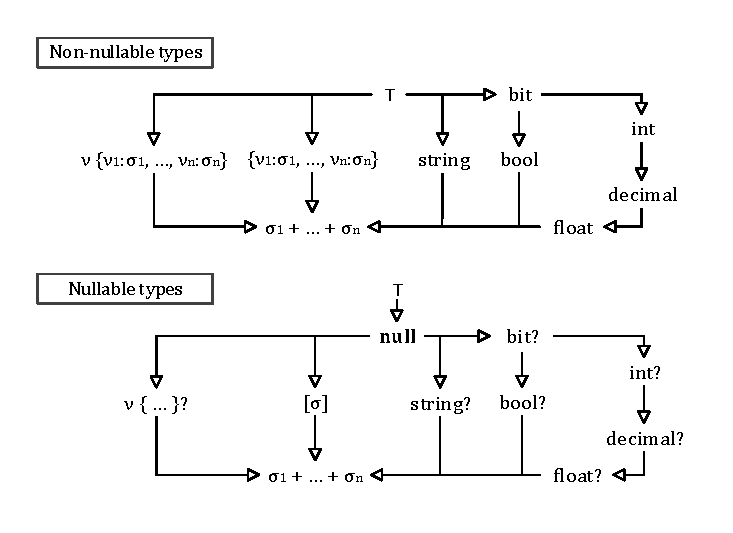
\includegraphics[scale=0.75,trim=5mm 5mm 5mm 5mm,clip]{images/hierarchy.pdf} % left bottom right top
\end{center}
\vspace{-0.5em}
\caption{Subtype relation between structural types}
\label{fig:subtyping-diagram}
\vspace{-0.5em}
\end{figure}

% -------------------------------------------------------------------------------------------------

\begin{figure*}[t]
\begin{equation*}
\hspace{3em}
\inference[(record-1)\;]
  { (\nu_i = \nu'_j \Leftrightarrow (i = j) \wedge (i \leq k))
      \qquad \forall i\in\{ 1 .. k \}.(\sigma_i \tsep \sigma'_i \vdash \sigma''_i) }
  { \begin{array}{l}
    \nu \; \{ \nu_1 : \sigma_1,  \; \ldots \;, \nu_k : \sigma_k, \; \ldots \;, \nu_n : \tau_n \} \tsep
    \nu \; \{ \nu'_1 : \sigma'_1, \; \ldots \;, \nu'_k : \sigma'_k, \; \ldots \;, \nu'_m : \tau'_m \} \vdash\\
    \nu \; \{ \nu_1 : \sigma''_1, \; \ldots \; , \nu_k : \sigma''_k, 
                            \nu_{k+1} : \addopt{\sigma_{k+1}}, \ldots, \nu_n : \addopt{\sigma_n},
                            \nu'_{k+1} : \addopt{\sigma'_{k+1}}, \ldots, \nu'_m : \addopt{\sigma'_m} \}
    \end{array} }
\end{equation*}

% union with something else
\begin{equation*}
\textnormal{\footnotesize{(union-1)}}\;\;
\inference
  {\exists i . \tytagof(\sigma_i) = \tytagof(\sigma) & \sigma \tsep \sigma_i \vdash \sigma_i' & \tytagof(\sigma)\neq\ident{union}}
  {\sigma \tsep (\sigma_1 + \ldots + \sigma_n) \vdash (\sigma_1 + \ldots + \dropopt{\sigma_i'} + \ldots + \sigma_n)}
\quad\quad
\inference
  {\nexists i . \tytagof(\sigma_i) = \tytagof(\sigma) & \tytagof(\sigma)\neq\ident{union}}
  {\sigma \tsep (\sigma_1 + \ldots + \sigma_n) \vdash (\sigma_1 + \ldots + \sigma_n + \dropopt{\sigma})}
\end{equation*}

% two union types
\begin{equation*}
\inference[(union-2)\;]
  { \tytagof(\sigma_i) = \tytagof(\sigma'_i) \quad 
    \sigma_i \tsep \sigma_i' \vdash \sigma''_i \qquad (\forall i\in \{ 1 .. k \}) }
  { \begin{array}{l}
    (\sigma_1  + \ldots + \sigma_k +  \ldots + \sigma_n) \tsep 
    (\sigma'_1 + \ldots + \sigma'_k + \ldots + \sigma'_m) \vdash\\
    (\sigma''_1 + \ldots + \sigma''_k + \sigma_{k+1} + \ldots + \sigma_{n} + \sigma'_{k+1} + \ldots + \sigma'_{m}) 
    \end{array} }
%
\qquad\quad
\inference[(union-3)\;]
  {(\textnormal{no other rule applies})}
  {\sigma_1 \tsep \sigma_2 \vdash \dropopt{\sigma_1} + \dropopt{\sigma_2}}
\end{equation*}

\begin{equation*}
\hspace{2em}
\inference[(order)\;]
  { \nu \; \{ \nu_1 : \sigma_1, \ldots, \nu_n : \sigma_n \} \tsep \sigma \vdash \sigma' }
  { \nu \; \{ \nu_{\pi(1)} : \sigma_{\pi(1)}, \ldots, \nu_{\pi(n)} : \sigma_{\pi(n)} \} \tsep \sigma \vdash \sigma' }
\quad
\inference
  { \sigma_1 + \ldots + \sigma_n \tsep \sigma \vdash \sigma' }
  { \sigma_{\pi(1)} + \ldots + \sigma_{\pi(n)} \tsep \sigma \vdash \sigma' }
\qquad (\pi~\textnormal{permutation})  
\end{equation*}


\begin{equation*}
\hspace{3em}
% collection types
\inference[(list)\;]
  {\sigma_1 \tsep \sigma_2 \vdash \sigma}
  {[\sigma_1] \tsep [\sigma_2] \vdash [\sigma]}
\qquad\qquad
% primitive types
\inference[(prim)\;]
  {\sigma_1 :> \sigma_2}
  {\sigma_1 \tsep \sigma_2 \vdash \sigma_1}\quad
\begin{array}{l}
  (\textnormal{when}\,~\sigma_1, \sigma_2 \in \{\ident{bit}, \ident{int}, \ident{decimal}, \ident{float} \} \\
   \quad~~\;\textnormal{or}\,~\sigma_1, \sigma_2 \in \{\ident{bit}, \ident{bool} \})
\end{array}   
\end{equation*}

% all rules are symmetric and reflexive
\begin{equation*}
\hspace{4.75em}
\inference[(sym)\;]
  {\sigma_1 \tsep \sigma_2 \vdash \sigma}
  {\sigma_2 \tsep \sigma_1 \vdash \sigma}
%
\qquad\quad
\begin{array}{l}
 \textnormal{\footnotesize{(refl)}}\;\; \sigma \tsep \sigma \vdash \sigma\\[0.75em]
 % top type
 \textnormal{\footnotesize{(top)}}\;\; \top \tsep \sigma \vdash \sigma
\end{array}
%
\qquad\quad 
% null and nullable
 \begin{array}{l}
 \textnormal{\footnotesize{(null-1)}}\;\; \sigma \tsep \kvd{null} \vdash \sigma \quad(\sigma :> \kvd{null}) \\[0.75em]
 \textnormal{\footnotesize{(null-2)}}\;\; \sigma \tsep \kvd{null} \vdash \sigma~\kvd{option} \quad(\sigma :\ngtr \kvd{null})
 \end{array}
\end{equation*}

\caption{Inference judgements that define the common supertype relation}
\label{fig:subtyping-cst}
\end{figure*}

% --------------------------------------------------------------------------------------------------

\noindent
Here is a summary of the key aspects of the definition:
\begin{itemize}
\item For numeric types (\ref{eq:sub-prim}), we infer a single most precise numeric type that 
  can represent all values from a sample dataset, so we order types by the ranges they represent;
  \ident{int} is a 32-bit integer, \ident{decimal} has a range of about $-1^{29}$ to $1^{29}$ and 
  \ident{float} is a double-precision floating-point.

\item The \ident{bit} type is a subtype of both \ident{int} and \ident{bool} (\ref{eq:sub-prim}). 
  Thus, a sample $0,1$ has a type \ident{bit}; $0,1,\kvd{true}$ is \ident{bool} and
  $0,1,2$ becomes \ident{int} (for a sample $0,1,2, \kvd{true}$ we would need a union type).

\item The \kvd{null} type is a subtype of all nullable types (\ref{eq:sub-null}), that is all 
  $\sigma$ types excluding non-nullable types $\hat{\sigma}$). Any non-nullable type is also a 
  subtype of its optional version (\ref{eq:sub-opt}).

\item There is a top type (\ref{eq:sub-top}), but no bottom type. It is possible to find common 
  supertype of any two types, because a union type $\tau_1 + \ldots + \tau_n$ is a supertype of all its 
  components (\ref{eq:sub-union-el}).

\item The remaining rules for unins are standard. Subtype can have fewer alternatives 
  (\ref{eq:sub-union1}), elements can be reordered (\ref{eq:sub-union2}) and subtyping is covariant 
  (\ref{eq:sub-union3}). Similarly, the collection type is also covariant (\ref{eq:sub-col}).

\item As usual, the subtyping on records is covariant (\ref{eq:sub-record1}), subtype can have additional 
  fields (\ref{eq:sub-record2}) and fields can  be reordered (\ref{eq:sub-record3}). The interesting rule 
  is the last one (\ref{eq:sub-record4}).  Together with covariance, it states that a subtype can omit some 
  fields, provided that their types are nullable.
\end{itemize}

\noindent
The rule that allows subtype to have fewer record elements (\ref{eq:sub-record4}) is particularly
important. It allows us to prefer records in some cases. For example, given two samples 
$\{ \ident{name}:\ident{string} \}$ and $\{ \ident{name}:\ident{string}, \ident{age}:\ident{int} \}$,
we can find a common supertype $\{ \ident{name}:\ident{string}, \ident{age}:\ident{int}~\kvd{option} \}$
which is also a record. For usability reasons, we prefer this to another common supertype
$\{ \ident{name}:\ident{string} \} + \{ \ident{name}:\ident{string}, \ident{age}:\ident{int} \}$.
The next section describes precisely how our inference algorithm works.

It is worth noting that some of the aspects (such as 3 different numeric types and handling of 
the \kvd{null} type) are specific to F\#. Similar problems will appear with most real-world
languages and systems. JVM and OCaml all haves multiple numeric types, but they would handle \kvd{null}
differently. 

We could also be more or less strict about missing data -- we choose to handle missing values 
silently when we can (\kvd{null} becomes an empty collection), but we are explicit in other cases 
(we infer \ident{string}~\kvd{option} as a hint to the user rather than treating \kvd{null} as an 
empty string). These choices are based on experience with using F\# Data in practice.

% -------------------------------------------------------------------------------------------------

\begin{figure*}
\begin{equation*}
\begin{array}{l}
 \ident{asInt}(i) \,\reduce i\\
 \ident{asInt}(d) \reduce i\quad(i = \lfloor d \rfloor)\\
 \ident{asInt}(f) \reduce i\quad(i = \lfloor f \rfloor) \\
 \ident{asInt}(t) \,\reduce i\quad(t~\text{\small represents}~i) \\
 \ident{asInt}(\kvd{true}) \reduce 1\\
 \ident{asInt}(\kvd{false}) \reduce 0\\
\end{array}
\;
\begin{array}{l}
 \ident{asDec}(i) \,\reduce d\quad(d = i)\\
 \ident{asDec}(d) \reduce d\\
 \ident{asDec}(f) \reduce d\quad(d = \lfloor f \rfloor) \\
 \ident{asDec}(t) \,\reduce d\quad(t~\text{\small represents}~d) \\
 \ident{asDec}(\kvd{true}) \reduce 1.0\\
 \ident{asDec}(\kvd{false}) \reduce 0.0\\
\end{array}
\;
\begin{array}{l}
 \ident{asFloat}(i) \,\reduce f\quad(f = i)\\
 \ident{asFloat}(d) \reduce f\quad(f = d)\\
 \ident{asFloat}(f) \reduce f\\
 \ident{asFloat}(t) \,\reduce f\quad(t~\text{\small represents}~f) \\
 \ident{asFloat}(\kvd{true}) \reduce 1.0\\
 \ident{asFloat}(\kvd{false}) \reduce 0.0\\
\end{array}
\;
\begin{array}{l}
 \ident{asStr}(i) \,\reduce t\quad(t~\text{\small represents}~i)\\
 \ident{asStr}(d) \reduce t\quad(t~\text{\small represents}~d)\\
 \ident{asStr}(f) \reduce t\quad(t~\text{\small represents}~f)\\
 \ident{asStr}(t) \,\reduce t\\
 \ident{asStr}(\kvd{true}) \reduce \str{true}\\
 \ident{asStr}(\kvd{false}) \reduce \str{false}\\
\end{array}
\end{equation*}
%
\begin{equation*}
\hspace{-1.5em}
\begin{array}{l}
 \ident{asBool}(1) \reduce \kvd{true}\\
 \ident{asBool}(1.0) \reduce \kvd{true}\\
 \ident{asBool}(\str{true}) \reduce \kvd{true}\\
 \ident{asBool}(\str{1}) \reduce \kvd{true}
 \\[0.6em]
 \ident{isNull}(\kvd{null}) \reduce \kvd{true} \\
 \ident{isNull}(\_) \reduce \kvd{false} 
\end{array}
\hspace{2.6em}
\begin{array}{l}
 \ident{asBool}(0) \reduce \kvd{false}\\
 \ident{asBool}(0.0) \reduce \kvd{false}\\
 \ident{asBool}(\str{false}) \reduce \kvd{false}\\
 \ident{asBool}(\str{0}) \reduce \kvd{false}\\
 \ident{asBool}(b) \reduce b
 \\[0.6em]
 \ident{getChildren}(\kvd{null}) \reduce [~]
\end{array}
\hspace{3.0em}
\begin{array}{l}
 \ident{getField}(\nu,\nu_i, \nu~\{\ldots, \nu_i=s_i, \ldots\}) \reduce s_i\\
 \ident{getField}(\bot, \nu_i, \{\ldots, \nu_i=s_i, \ldots\}) \reduce s_i\\
 \ident{getField}(\nu,\nu', \nu~\{\ldots, \nu_i=s_i, \ldots\}) \reduce \kvd{null}\quad(\nexists i.\nu_i=\nu' )\\
 \ident{getField}(\bot, \nu', \{\ldots, \nu_i=s_i, \ldots\}) \reduce \kvd{null}\quad(\nexists i.\nu_i=\nu' )
 \\[0.6em]
 \ident{getChildren}([s_1; \ldots; s_n]) \reduce [s_1; \ldots; s_n]
\end{array}
\end{equation*}
%
\begin{equation*}
\hspace{-1.5em}
\begin{array}{l}
 \ident{isTag}(\ident{string}, t) \reduce \kvd{true} \\
 \ident{isTag}(\ident{bool}, v) \reduce \kvd{true} \quad(\textnormal{when}~v\in{0,1,0.0, 1.0, \kvd{true},\kvd{false}} )\\
 \ident{isTag}(\ident{number}, v) \reduce \kvd{true} \quad(\textnormal{when}~v=i, v=d, v=f) \\
 \ident{isTag}(\ident{collection}, [s_1; \ldots; s_n]) \reduce \kvd{true} \\
\end{array}
\hspace{1.8em}
\begin{array}{l}
 \ident{isTag}(\ident{collection}, \kvd{null}) \reduce \kvd{true} \\
 \ident{isTag}(\ident{rec-anon}, \{ \nu_1\mapsto s_1, \ldots, \nu_n\mapsto s_n \}) \reduce \kvd{true} \\
 \ident{isTag}(\ident{rec-named}~\nu, \nu\;\{ \nu_1\mapsto s_1, \ldots, \nu_n\mapsto s_n \}) \reduce \kvd{true} \\
 \ident{isTag}(\_, \_) \reduce \kvd{false} \\
\end{array}
\end{equation*}

\caption{Reduction rules for conversion functions}
\label{fig:op-conversions}
\end{figure*}

% -------------------------------------------------------------------------------------------------

\subsection{Common supertype relation}
\label{sec:inference-commonsuper}

As mentioned earlier, the structured type inference relies on a finding common supertype. However,
the partially ordered set of types does not have a unique greatest lower bound. For example, record types
$\{\ident{a}:\ident{int}\}$ and $\{\ident{b}:\ident{bool}\}$ have common supertypes
$\{\ident{?a}:\ident{int}, \ident{?b}:\ident{bool}\}$ and $\{\ident{a}:\ident{int}\} + \{\ident{b}:\ident{bool}\}$
which are unrelated. Our inference algorithm always prefers records over unions (Theorem~\ref{thm:no-unions}). 
The definition of the \emph{common supertype} relation uses a number of auxiliary definitions 
that are explained in the discussion that follows.

\begin{definition}
A \emph{common supertype} of types $\sigma_1$ and $\sigma_2$ is a type $\sigma$, written 
$\sigma_1 \triangledown \sigma_2 \vdash \sigma$, obtained according to the inference rules in 
Figure~\ref{fig:subtyping-cst}.
\end{definition}

\noindent
When finding a common supertype of two records (\emph{record-1}), we return a record type that has the union
of fields of the two arguments. We assume that the names of the first $k$ fields are the same and the
remaining fields have different names. To get a record with the right order of elements, we provide the
(\emph{order}) rule. The types of shared fields become common supertypes of their 
respective types (recursively). Fields that are present in only one record are marked as optional using
the following helper definition:
%
\begin{equation*}
\begin{array}{rcll}
 \addopt{\hat{\sigma}} &\narrow{=}& \hat{\sigma}~\kvd{option} \qquad&(\textnormal{non-nullable types})\\
 \addopt{\sigma} &\narrow{=}& \sigma &(\textnormal{otherwise})
\end{array}
\end{equation*}
%
Finding a common supertype of when one type is a union is more complicated. Our definiion aims to 
use a flat structure (avoid nesting unions) and limit the number of cases. This is done by grouping
types that have a common supertype which is not a union type. For example, rather than inferring 
$\ident{int} + (\ident{bool} + \ident{decimal})$, our algorithm will find the common supertype of
$\ident{int}$ and $\ident{decimal}$ (which is \ident{decimal}) and it will produce just $\ident{decimal}+\ident{bool}$.

To identify which types have a common supertype which is not a union, we group the types by a 
\emph{tag}, which is defined as:
%
\begin{equation*}
\begin{array}{rcl}
 \tytag &\narrow{=}&  \ident{string} \lsep \ident{bool} \lsep \ident{number} \lsep \ident{union} \lsep \ident{collection} \\
        &\narrow{\lsep}& \ident{rec-anon} \lsep \ident{rec-named}\;~\nu 
\end{array}
\end{equation*}
%
The tag of a type is obtained using a function $\tytagof{(-)} : \sigma \rightarrow \tytag$:
%
\begin{equation*}
\begin{array}{rcl}
 \tytagof(\ident{string}) &\narrow{=}& \ident{string}\\
 \tytagof(\ident{bool}) &\narrow{=}& \ident{bool}\\
 \tytagof(\ident{decimal}) = \tytagof(\ident{float}) &\narrow{=}& \ident{number}\\
 \tytagof(\ident{int}) = \tytagof(\ident{bit}) &\narrow{=}& \ident{number}\\
 \tytagof([\sigma]) &\narrow{=}& \ident{collection}\\
\end{array}
\end{equation*}
\begin{equation*}
\begin{array}{rcl}
 \tytagof(\sigma + \ldots + \sigma) &\narrow{=}& \ident{union}\\
 \tytagof(\{ \nu_1 : \sigma_1, \; \ldots \; , \nu_n : \sigma_n \}) &\narrow{=}& \ident{rec-anon}\\
 \tytagof(\nu\; \{ \nu_1 : \sigma_1, \; \ldots \; , \nu_n : \sigma_n \}) &\narrow{=}& \ident{rec-named}~\nu \\
 \tytagof(\hat{\sigma}~\kvd{option}) &\narrow{=}& \tytagof(\hat{\sigma})
\end{array}
\end{equation*}
%
The function is undefined for the $\top$ and $\kvd{null}$ types, but this is not a 
problem because these types never need to be used as arguments in Figure~\ref{fig:subtyping-cst}.
The $\top$ type is always eliminated using the (\emph{top}) rule and the \kvd{null} type
is eliminated using either (\emph{null-1}) or (\emph{null-2}).

The handling of unions is specified using three rules. When adding a non-union type to a 
union (\emph{union-1}), the union may or may not contain a case with the same tag as the new type.
If it does, the new type is combined with the existing one, otherwise a new case is added.
When combining two unions (\emph{union-2}), we group the cases that have a shared tags.
Finally, the last rule (\emph{union-3}) covers the case when we are combining two non-union types.
As discussed earlier, union implicitly permits \kvd{null} values and so we use the following 
auxiliary function which makes nullable types non-nullable (when possible) to simplify the type:
%
\begin{equation*}
\begin{array}{rcll}
 \dropopt{\hat{\sigma}~\kvd{option}} &\narrow{=}& \hat{\sigma} &(\textnormal{option})\\
 \dropopt{\sigma} &\narrow{=}& \sigma &(\textnormal{otherwise})
\end{array}
\end{equation*}
%
The remaining rules are straightforward. For collections, we find the common supertype of 
its elements (\emph{list}); for compatible primitive types, we choose one of the two (\emph{prim})
and a common supertype with \kvd{null} is either the type itself (\emph{null-1}) or an option 
 (\emph{null-2}).

\paragraph{Properties.}
The common supertype relation finds a single supertype (among multiple candidates).
The following theorems specify that the found type is uniquely defined (up to reordering of 
fields in records and union cases) and is, indeed, a common supertype.
%
\begin{theorem}[Uniqueness]
\raggedright
If $\sigma_1 \triangledown \sigma_2 \vdash \sigma$ and $\sigma_1 \triangledown \sigma_2 \vdash \sigma'$
then it holds that $\sigma :> \sigma'$ and $\sigma' :> \sigma$.
\end{theorem}
\begin{proof}
The assumptions and shapes of the types to be unified in the rules in Figure~\ref{fig:subtyping-cst} 
are disjoint, with the exception of (\emph{order}), (\emph{sym}) and (\emph{refl}). These rules 
always produce types that are subtypes of each other. This property is preserved by rules that use the
common supertype relation recursively.
\end{proof}

\begin{theorem}[Common supertype]
\raggedright
If $\sigma_1 \triangledown \sigma_2 \vdash \sigma$ then it holds that $\sigma :> \sigma_1$ and $\sigma :> \sigma_2$.
\end{theorem}
\begin{proof}
By induction over the common supertype derivation $\vdash$.
\end{proof}

\noindent
We stated earlier that the common supertype relation minimises the use of union types 
(by preferring common numeric types or common record types when possible). This property
can be stated and proved formally:
%
\begin{theorem}
\label{thm:no-unions}
Given $\sigma_1, \sigma_2$ if there is s $\sigma$ such that $\sigma :> \sigma_1$ and 
$\sigma :> \sigma_2$ and $\sigma$ is not a union type, then $\sigma_1 \tsep \sigma_2 \vdash \sigma'$ 
and $\sigma'$ is not a union type.
\end{theorem}
\begin{proof}
The only rule that introduces an union type is (\emph{union-3}), which is used only when 
no other inference rule can be applied.
\end{proof}

% ==================================================================================================

\section{Formalising type providers}
\label{sec:formal}

In this section, we build the necessary theoretical framework for proving the relativised type safety 
property of F\# Data type providers in Section~\ref{sec:safety}. We start by discussing the runtime 
representation of structured values and runtime conversions (Section~\ref{sec:formal-convert}). Then 
we embed these into a formal model of an F\# subset that is necessary for discussing type providers 
(Section~\ref{sec:formal-ff}) and we describe how F\# Data type providers turn an inferred 
structural type into actual F\# code (Section~\ref{sec:formal-tp}).

% -------------------------------------------------------------------------------------------------

\subsection{Structural values and conversions}
\label{sec:formal-convert}

In the model presented here, we represent JSON, XML and CSV documents using the same 
\emph{structural value}\footnote{Here, we diverge from the actual implementation in F\# Data which 
uses a different implementation for each format (reusing existing libraries).}. Structural values are 
first-order and can be one of the primitive values (Boolean, string, integer, decimal and float), a 
missing value (\kvd{null}), a collection and a record (named or unnamed):
%
\begin{equation*}
\begin{array}{lcl}
 s  &\narrow{=}& i \lsep d \lsep f \lsep t \lsep \kvd{true} \lsep \kvd{false} \lsep \kvd{null} \\[0.1em]
    &\narrow{|}& [s_1; \ldots; s_n] \\[0.1em]
    &\narrow{|}& \{ \nu_1 \mapsto s_1, \ldots, \nu_n \mapsto s_n \}\\[0.1em]
    &\narrow{|}& \nu~\{ \nu_1 \mapsto s_1, \ldots, \nu_n \mapsto s_n \} \\
\end{array}
\end{equation*}

\noindent
The first few cases represent primitive values ($i$ for integers, $d$ for decimals, $f$ for floating
point numbers and $t$ for strings). A collection is written as a list of values in square brackets, 
separated by semicolons. A record can optionally start with its name $\nu$, followed by a sequence of 
field assignments $\nu_i \mapsto s_i$ written in curly brackets.

As suggested by subtyping, our system permits certain runtime conversions (\emph{e.g.}~a numerical 
value \num{1} can be treated as \kvd{true}). These are captured by the following operations:
%
\begin{equation*}
\begin{array}{lcl}
 op &\narrow{=}& \ident{asInt}(s) \lsep \ident{asDec}(s) \lsep \ident{asFloat}(s) \lsep \ident{asBool}(s)  \\
    &\narrow{|}& \ident{asStr}(s) \lsep \ident{getChildren}(s) \lsep \ident{getField}(\nu_{\ident{opt}}, \nu, s)\\
    &\narrow{|}& \ident{isNull}(s) \lsep \ident{isTag}(t, s)
\end{array}
\end{equation*}
%
The reduction rules for these operations are defined in Figure~\ref{fig:op-conversions}. It is important
to note that the relativised property we prove about F\# Data specifies \emph{sufficient}, but
not \emph{necessary} conditions. That is, a type provided based on a sample is guaranteed to work 
correctly on certain inputs, but may also handle several additional inputs.

The conversion functions follow this approach. They perform conversions required by the subtyping relation
(\emph{e.g.}~integer is converted to decimal or a float) but also attempt additional conversions.

\begin{itemize}
\item \textbf{Widening operations.} The widening operations are required by the subtyping. These include
  converting to a wider numerical type (integer to decimal and float, decimal to float, converting 0 and 
  1 to Boolean).

\item \textbf{Conversions.} Additional conversions are not strictly required, but prove useful in practice.
  These include converting to a smaller numerical type (such as float to integer) written as $i=\lfloor f\rfloor$,
  which is not defined in case of arithmetic overflow; conversion to and from string values written as
  ``$t$~represents~$i$'', which parses or formats a non-string value and also trating of decimals 
  0.0 and 1.0 as Booleans.

\item \textbf{Structural operations.} Aside from primitives, the \ident{getChildren} operation returns treats
  \kvd{null} as an empty collection. The \ident{getField} function is defined separately for named and unnamed
  records (we write $\bot$ for a name of an unnamed record). Accessing a field of a named record checks that 
  the expected record name matches the actual.

\item \textbf{Helper functions.} The semantics also defines two helper functions. The \ident{isNull} function
  is used to check whether value is \kvd{null} and \ident{isTag} is used to test whether a value can be treated 
  as a value of type associated with the specified tag (as defined in Section~\ref{sec:inference-commonsuper}).
  The last line defines a ``catch all'' pattern, which returns \kvd{false} for all remaining cases.
\end{itemize}

% -------------------------------------------------------------------------------------------------

\begin{figure}
\begin{equation*}
\begin{array}{rl}
 \textnormal{\footnotesize{(member)}}&
 \hspace{-0.4em}
 \inference
 { \kvd{type}~C(\overline{x:\tau})=\ldots \kvd{member}~N_i : \tau_i = e_i \ldots }
 { (\kvd{new}~C(\overline{v})).N_i \reduce e_i[\overline{x} \leftarrow \overline{v}] }\\
 \\
 \textnormal{\footnotesize{(ctx)}}&
 \hspace{-0.4em}
  E[e] \reduce E[e'] \qquad\qquad(\textnormal{when}~e \reduce e')\\
 \\
 \textnormal{\footnotesize{(cond1)}}&
 \hspace{-0.4em}
 \kvd{if}~\kvd{true}~\kvd{then}~e_1~\kvd{else}~e_2 ~\reduce~ e_1 \\
 \\
 \textnormal{\footnotesize{(cond2)}}&
 \hspace{-0.4em}
 \kvd{if}~\kvd{false}~\kvd{then}~e_1~\kvd{else}~e_2 ~\reduce~ e_2 \\
 \\
 \textnormal{\footnotesize{(match1)}}&
 \hspace{-1em}
 \begin{array}{l}
  \kvd{match}~\ident{None}~\kvd{with} \\
  \ident{Some}(x) \rightarrow e_1 \,|\, \ident{None} \rightarrow e_2
 \end{array} \hspace{-0.5em} ~\reduce~ e_2 \\
 \\
 \textnormal{\footnotesize{(match2)}}&
 \hspace{-1em}
 \begin{array}{l}
    \kvd{match}~\ident{Some}(v)~\kvd{with} \\
    \ident{Some}(x) \rightarrow e_1 \,|\, \ident{None} \rightarrow e_2
 \end{array} \hspace{-0.5em} ~\reduce~ e_1[x\leftarrow v]\\
 \\
 \textnormal{\footnotesize{(match3)}}&
 \hspace{-1em}
 \begin{array}{l}
  \kvd{match}~[v_1;\ldots;v_n]~\kvd{with} \\[0em]
  [x_1;\ldots;x_m ] \rightarrow e_1 \,|\, \_ \rightarrow e_2
 \end{array} \hspace{-0.5em} ~\reduce~ e_2\quad(m\neq n) \\
 \\
 \textnormal{\footnotesize{(match4)}}&
 \hspace{-1em}
 \begin{array}{l}
  \kvd{match}~[v_1;\ldots;v_n]~\kvd{with} \\[0em]
  [x_1;\ldots;x_n ] \rightarrow e_1 \,|\, \_ \rightarrow e_2
 \end{array} \hspace{-0.5em} ~\reduce~ e_1[\overline{x}\leftarrow\overline{v}] \\
 \\
 \textnormal{\footnotesize{(map)}}&
 \hspace{-0.4em}
 \ident{List.map}~(\lambda x.e)~[v_1; \ldots] ~\reduce~ [e[x\leftarrow v_1]; \ldots] \\
\end{array}
\end{equation*}

\caption{Remaining reduction rules for Featherweight F\#}
\label{fig:ff-reduction}
\vspace{-0.5em}
\end{figure}

% -------------------------------------------------------------------------------------------------

\subsection{Featherweight F\#}
\label{sec:formal-ff}

The semantics fragment introduced in the previous section discusses values and operations that are used by
F\# Data. This section adds a minimal subset of the standard F\# language. We focus on the object system
(which is what F\# type providers produce) and so the following is based on Featherweight Java. However, we
only need class types (without inheritance) with properties. A class has a single implicit constructor and 
the declaration closes over constructor parameters. In addition, we include special constructs for working
with option types and lists.
%
\begin{equation*}
\begin{array}{rcl}
 \tau &\narrow{=}& \ident{int} \lsep \ident{decimal} \lsep \ident{float} \lsep \ident{bool} \lsep \ident{string} \\[0.0em]
      &\narrow{|}& C \lsep \ident{StructVal} \lsep \ident{list}\langl\tau\rangl \lsep \ident{option}\langl\tau\rangl \\[0.6em]
 L &\narrow{=}& \kvd{type}~C(\overline{x:\tau}) = \overline{M} \\[0.0em]
 M &\narrow{=}& \kvd{member}~N:\tau=e \\[0.6em]
 v &\narrow{=}& s \lsep \ident{None} \lsep \ident{Some}(v) \lsep \kvd{new}~C(\overline{v}) \\[0.0em]
 e &\narrow{=}& op \lsep e.N \lsep \kvd{new}~C(\overline{e}) \lsep {\kvd{if}~e_1~\kvd{then}~e_2~\kvd{else}~e_3}\\
   &\narrow{|}& \ident{Some}(e)\lsep\kvd{match}~e~\kvd{with}~\ident{Some}(x) \rightarrow e_1 \,|\, \ident{None} \rightarrow e_2 \\
   &\narrow{|}& \kvd{match}~e~\kvd{with}~[x_1; \ldots; x_n] \rightarrow e_1 \,|\, \_ \rightarrow e_2 \\
   &\narrow{|}& [e_1;\ldots;e_n]\lsep \ident{List.map}~(\lambda x\rightarrow e_1)~e_2
\end{array}
\end{equation*}

\noindent
In the above definition, $\tau$ denotes types including a special type \ident{StructVal} for all structural 
values $s$; a class definition $L$ consists of a constructor and zero or more members. Values $v$ include 
previously defined structural values $s$ and values for the option type; finally expressions $e$ include all 
previously defined operations $op$, class construction, member access, conditionals and expressions for working 
with option values and lists. We include \ident{List.map} as a special construct to avoid making the language too complex.

In this paper, we do not define the typing of the F\# subset introduced above as our goal is not to prove
type safety for the core language. For the relativized soundness proof in Section~\ref{sec:safety}, it is
sufficient to discuss reduction.

\paragraph{Reduction.} The reduction relation is of the form $e \reduce e'$. We also write 
$e \reduce^{*} e'$ to denote the reflexive and transitive closure of $\reduce$. The reduction rules
for primitive functions $op$ were discussed earlier in Figure~\ref{fig:op-conversions}. The rules 
for other expressions defined above are provided in Figure~\ref{fig:ff-reduction}.

The (\emph{ctx}) rule performs a reduction inside a sub-expression specified by an evaluation context.
This models the eager evaluation order of F\#. An evaluation context $E$ is defined as:

\noindent
\begin{equation*}
\begin{array}{rcl}
 E &\narrow{=}& f(E) \lsep E.N \lsep \kvd{new}~C(\overline{v}, E, \overline{e}) \lsep \kvd{if}~E~\kvd{then}~e_1~\kvd{else}~e_2 \\[0.1em]
   &\narrow{|}& \ident{Some}(E) \lsep \kvd{match}~E~\kvd{with}~\ident{Some}(x) \rightarrow e_1 \,|\, \ident{None} \rightarrow e_2 \\[0.1em]
   &\narrow{|}& [\overline{v};E;\overline{e}] \lsep \kvd{match}~E~\kvd{with}~[x_1; \ldots; x_n] \rightarrow e_1 \,|\, \_ \rightarrow e_2 \\[0.1em]
   &\narrow{|}& \ident{map}~(\lambda x\rightarrow e)~E \lsep [\cdot] 
 \\[0.6em]
 f &\narrow{\in}& \{\; \ident{asInt}, \ident{asDec}, \ident{asFloat}, \ident{asBool}, \ident{asStr}, \\[0.1em]
              && ~~\; \ident{getField}, \ident{getChildren}, \ident{isNull}, \ident{isTag} \;\}
\end{array} 
\end{equation*}

\noindent
The evaluation first reduces arguments of functions and the evaluation proceeds from left to right 
as denoted by $\overline{v}, E, \overline{e}$ in constructor arguments or $\overline{v};E;\overline{e}$
in list initialization.

We write $e[\overline{x} \leftarrow \overline{v}]$ for the result of replacing variables $\overline{x}$ by
values $\overline{v}$ in expression. The (\emph{member}) rule reduces a member access using a class 
definition in the assumption to obtain the body of the expression. Finally, the remaining six rules
provide standard reductions for conditionals and pattern matching.

The language is sufficient for our purpose, but simple. It does not provide recursion
and so all expressions reduce to a value in a finite number of steps or get stuck due to an error
condition. An error condition can be a wrong argument passed to conditional, pattern matching or
one of the conversion functions from Figure~\ref{fig:op-conversions}.

% -------------------------------------------------------------------------------------------------

\begin{figure*}
\begin{multicols}{2}
% Primitive structural types become corresponding F# types and conversion is inserted
\noindent
\begin{equation*}
\begin{array}{l}
 \sem{\sigma_p}_e = \tau_p,op(e),\emptyset\quad\textnormal{where} \\[0.4em]
\quad\sigma_p, \tau_p, op\in  \{~ (\ident{bit}, \ident{bool}, \ident{asBool}),  (\ident{bool}, \ident{bool}, \ident{asBool})\\[0.2em]
\hspace{2.9em} (\ident{int}, \ident{int}, \ident{asInt}), (\ident{decimal},\ident{decimal},\ident{asDec}),\\[0.2em]
\hspace{2.9em} (\ident{float},\ident{float},\ident{asFloat}), (\ident{string},\ident{string},\ident{asStr}) ~\}\\[0.6em]
\end{array}
\end{equation*}
%
% Records become classes
\begin{equation*}
\begin{array}{l}
 \sem{\nu_{\ident{opt}}\; \{ \nu_1 : \sigma_1, \ldots, \nu_n : \sigma_n \}}_e = \\[0.1em]
 \quad C, \kvd{new}~C(e), L_1\cup\ldots\cup L_n\cup\{ L \}\quad\textnormal{where}\\[0.6em]
 \qquad \;\;C~\textnormal{is a fresh class name} \\[0.1em]
 \qquad \;\,\,L = \kvd{type}~C(v:\ident{StructVal})~=~M_1\ldots M_n  \\[0.1em]
 \qquad M_i = \kvd{member}~\nu_i:\tau_i=e_i\\[0.1em]
 \qquad \tau_i, e_i, L_i = \sem{\sigma_i}_{e'},\;\; e'=\ident{getField}(\nu_{\ident{opt}}, \nu_i, e)\\[0.6em]
\end{array}
\end{equation*}
%
% Collections
\begin{equation*}
\begin{array}{l}
 \sem{\,[\sigma]\,}_e = \ident{list}\langl\tau\rangl, \ident{List.map}~(\lambda x\rightarrow e')~(\ident{getChildren}(e)), L\\[0.4em]
 \quad \textnormal{where}~~\tau, e', L = \sem{\hat{\sigma}}_x
\end{array}
\end{equation*}

% Option values
\noindent
\begin{equation*}
\begin{array}{l}
 \sem{\hat{\sigma}\;\,\kvd{option}}_e = \\[0.2em]
 \hspace{1.25em} \ident{option}\langl\tau\rangl, \kvd{if}~\ident{isNull}~e~\kvd{then}~\ident{None}~\kvd{else}~\ident{Some}(e'), L\\[0.2em] 
 \hspace{1.25em} \textnormal{where}~\tau, e', L = \sem{\hat{\sigma}}_e
\end{array}
\end{equation*}
%
% Sum type
\begin{equation*}
\begin{array}{l}
 \sem{\sigma_1 + \ldots + \sigma_n}_e = \\[0.1em]
 \quad C, \kvd{new}~C(e), L_1\cup\ldots\cup L_n\cup\{ L \}\quad\textnormal{where}\\[0.6em]
 \qquad \;\;C~\textnormal{is a fresh class name} \\[0.1em]
 \qquad \;\,\,L = \kvd{type}~C(v:\ident{StructVal})~=~M_1\ldots M_n \\[0.1em]
 \qquad M_i = \kvd{member}~\nu_i:\ident{option}\langl\tau_i\rangl=\\[0.1em]
 \hspace{5.8em}  \kvd{if}~\ident{isNull}(v)~\kvd{then}~\ident{None}~\kvd{else} \\
 \hspace{5.8em}  \kvd{if}~\ident{isTag}(t_i, v)~\kvd{then}~
     \ident{Some}(e_i)~\kvd{else}~\ident{None} \\[0.1em]
 \qquad \tau_i, e_i, L_i = \sem{\sigma_i}_e,\;\; t_i = \tytagof{(\sigma_i)},\;\; \nu_i=\nameoftag{(t_i)}
\end{array}
\end{equation*}
%
% Anything else
\begin{equation*}
\begin{array}{l}
 \sem{\top}_v = \sem{\kvd{null}}_v = \ident{StructVal}, v, \emptyset
\end{array}
\end{equation*}
\end{multicols}

\vspace{-0.5em}
\noindent
\begin{equation*}
\qquad
\qquad
\begin{array}{rcl}
 \nameoftag(\ident{string}) &\narrow{=}& \ident{String} \\
 \nameoftag(\ident{bool}) &\narrow{=}& \ident{Boolean} \\
\end{array}
\qquad
\begin{array}{rcl}
 \nameoftag(\ident{number}) &\narrow{=}& \ident{Number} \\
 \nameoftag(\ident{collection}) &\narrow{=}& \ident{List} \\
\end{array}
\qquad
\begin{array}{rcl}
 \nameoftag(\ident{rec-anon}) &\narrow{=}& \ident{Record} \\
 \nameoftag(\ident{rec-named}\;\nu) &\narrow{=}& \nu \\
\end{array}
\end{equation*}

\caption{Type provider -- generation of featherweight F\# types from inferred structural types}
\label{fig:tp-generation}
\vspace{-0.5em}
\end{figure*}

% -------------------------------------------------------------------------------------------------

\subsection{Type providers}
\label{sec:formal-tp}

So far, we defined the type inference algorithm for structured data formats which produces a structured
type $\sigma$ based on one or more sample documents (Section~\ref{sec:inference}). In Section~\ref{sec:formal-ff},
we defined a simplified model of F\# language and evaluation, which also included conversions that
model the F\# Data library runtime (Section~\ref{sec:formal-tp}). In this section, we define how
the type providers work, which links the two aspects discussed so far.

The type providers for XML, CSV and JSON all work in the same way. They take sample documents and infer a common
supertype $\sigma$ from the samples. From $\sigma$, they then generate F\# types that are then exposed to the
programmer\footnote{The actual implementation provides \emph{erased types} as described in [?]. Here, we treat
the code as actually generated. This is an acceptable simplification, because F\# Data type providers do not 
rely on laziness that is available through erased types.}. 

\paragraph{Type provider mapping.}
When generating types, the type provider produces an F\# type $\tau$, expression that wraps a structured 
document value (of type \ident{StructVal}) as a value of type $\tau$ and a collection of class definitions. 
We express it using the following mapping:
%
\begin{equation*}
\sem{-}_e : \sigma \rightarrow \tau \times e' \times L
\end{equation*}
%
The semantics is parameterized by an expression $e$, which represents code to obtain a structured value that is
being wrapped. Then, given an inferred structured type $\sigma$, the type provider produces an F\# type $\tau$,
an expression $e'$ which constructs a value of type $\tau$ using $e$ and also a set of class definitions $L$.

Figure~\ref{fig:tp-generation} shows the rules that define $\sem{-}_e$. Primitive types are all
handled by a single rule. For a given structural type, it returns the corresponding F\# type -- the types are
mapped directly with the exception of \ident{bit}, which becomes an F\# \ident{bool}. The generated code calls
an appropriate conversion function from Figure~\ref{fig:op-conversions} on the input.

Handling of records is more interesting. We generate a new class $C$ that takes a structured value as constructor
parameter. For each record field, we generate a new member with the same name as the field\footnote{The actual
F\# Data implementation also capitalizes the names.} The body of the member calls \ident{getField} and then
passes this expression to $\sem{\sigma_i}$ which adds additional wrapping that maps the field (structured value
of type $\sigma_i$) into an F\# type $\tau_i$. The returned expression creates a new instance of $C$ and
the mapping returns the class $C$ together with all recursively generated definitions.

A collection type becomes an F\# $\ident{list}\langl\tau\rangl$. The returned expression calls \ident{getChildren}
(which turns \kvd{null} values into empty lists) and then uses \ident{List.map} to convert all nested values to 
an F\# type $\tau$. The handling of option type is similar -- it checks if the original value is \kvd{null} and
if no, it wraps the recursively generated conversion expression $e'$ in the \ident{Some} constructor.

As discussed earlier, union types are also generated as classes with properties. Given a union type $\sigma_1 + \ldots + \sigma_n$,
we get corresponding F\# types $\tau_i$ and generate $n$ members of type $\ident{option}\langl \tau_i\rangl$.
Each member return \ident{Some} when the value is not \kvd{null} and has the right structure (checked by 
\ident{isTag}). The type inference algorithm also guarantees that there is only one case for each type tag 
(Section~\ref{sec:inference-commonsuper}) and there are no nested union types. Thus, checking for a tag is
sufficient and we can also use the tag to identify the name of the generated member (using the
\ident{nameof} function).

\paragraph{Example 1.}
To illustrate how the type provision mechanism works, we now consider two simple examples. First, assume 
that the inferred type is a record with two fields (one optional) such as 
$\ident{Person}~\{~\ident{Age}:\ident{int}~\kvd{option}, \ident{Name}:\ident{string}~ \}$. Applying the
rules from Figure~\ref{fig:tp-generation} produces the following class:
%
\begin{equation*}
\begin{array}{l}
 \kvd{type}~\ident{Person}(\ident{v}:\ident{StructVal})~= \\[0.1em]
 \quad \kvd{member}~\ident{Age}~:~\ident{option}\langl\ident{int}\rangl~= \\[0.1em]
 \qquad \kvd{if}~\ident{isNull}~(\ident{getField}(\ident{Person},\ident{Age}, \ident{v}))~\kvd{then}~\ident{None} \\[0.1em]
 \qquad \kvd{else}~\ident{Some}(\ident{asInt}(\ident{getField}(\ident{Person},\ident{Age}, \ident{v}))) \\[0.1em]
 \quad \kvd{member}~\ident{Name}~:~\ident{string}~= \\[0.1em]
 \qquad \ident{asStr}(\ident{getField}(\ident{Person},\ident{Name}, \ident{v}))
\end{array}
\end{equation*}
%
The body of the \ident{Age} member is produced by the case for optional types applied to an expression
$\ident{getField}(\ident{Person},\ident{Age},v)$. If the returned field is not \kvd{null}, then the member
calls \ident{asInt} (produced by the case for primitive types) and wraps the result in the \ident{Some}
constructor. Note that \ident{getField} is defined even when the field does not exist, but returns \ident{null}.
This lets us treat missing fields as optional fields. The \ident{Name} member is similar, but does not 
perform any checks. 

For completeness, a type corresponding to the record is \ident{Person} and given a 
structural document $s$, we create a \ident{Person} value by calling $\kvd{new}~\ident{Person}(s)$.

\paragraph{Example 2.} The second example illustrates the remaining parts of the type provision,
including collections and union types. Teusing the \ident{Person} type from the previous example,
consider a collection $[\ident{Person}+\ident{string}]$, which contains a mix of \ident{Person} and string values.

\noindent
\begin{equation*}
\begin{array}{l}
 \kvd{type}~\ident{PersonOrString}(\ident{v}:\ident{StructVal})~= \\[0.1em]
 \quad \kvd{member}~\ident{Person}~:~\ident{option}\langl\ident{Person}\rangl~= \\[0.1em]
 \qquad \kvd{if}~\ident{isNull}(v)~\kvd{then}~\ident{None}~\kvd{else} \\[0.1em]
 \qquad \kvd{if}~\ident{isTag}(\ident{rec-named Person}, v)~\kvd{then}~\\[0.1em]
 \qquad\quad \ident{Some}(\kvd{new}~\ident{Person}(v))~\kvd{else}~\ident{None} \\[0.1em]
 \quad \kvd{member}~\ident{String}~:~\ident{option}\langl\ident{string}\rangl~= \\[0.1em]
 \qquad \kvd{if}~\ident{isNull}(v)~\kvd{then}~\ident{None}~\kvd{else} \\[0.1em]
 \qquad \kvd{if}~\ident{isTag}(\ident{string}, v)~\kvd{then}~\\[0.1em]
 \qquad\quad \ident{Some}(\ident{asStr}(v))~\kvd{else}~\ident{None}
\end{array}
\end{equation*}

\noindent
The type provider generates the above type and the collection type is mapped to an F\# type 
$\ident{list}\langl\ident{PersonOrString}\rangl$. Given a structural document value $s$, the code
to obtain the wrapped F\# value is:
%
\begin{equation*}
\ident{List.map}~(\lambda x\rightarrow\kvd{new}~\ident{PersonOrString}(x))~(\ident{getChildren}(s))
\end{equation*}
%
The \ident{PersonOrString} type contains one property for each of the union case. In the body, they
check that the value is not \kvd{null} and that it has the right structure (using the \ident{isTag}
function). This checks that the value is a record named \ident{Person} or a string, respectively.
If the conditions are satisfied, the value is converted to the F\# type corresponding to the case
and wrapped in \ident{Some}.

% --------------------------------------------------------------------------------------------------

\subsection{Infering types from values}

Before concluding the section on formalizing type providers, 


\begin{equation*}
\begin{array}{rclcrcl}
 \semalt{0} &\narrow{=}& \ident{bit} &\qquad& \semalt{1} &\narrow{=}& \ident{bit} \\
 \semalt{i} &\narrow{=}& \ident{int} && \semalt{d} &\narrow{=}& \ident{decimal} \\
 \semalt{f} &\narrow{=}& \ident{float} && \semalt{t} &\narrow{=}& \ident{string} \\
 \semalt{b} &\narrow{=}& \ident{bool} && \semalt{\kvd{null}}  &\narrow{=}& \kvd{null} \\[0em]
\end{array}
\end{equation*}
\noindent
\begin{equation*}
\begin{array}{l}
 \semalt{[s_1; \ldots; s_n]} = [\sigma_n] \quad\textnormal{where}\\[0.1em]
 \qquad\sigma_0 = \top,~ \forall i\in \{ 1.. n \}.~ \sigma_{i-1} \triangledown \semalt{s_i} \vdash \sigma_i
 \\[0.6em]
 \semalt{\nu_{\ident{opt}}~\{ \nu_1 \mapsto s_1, \ldots, \nu_n \mapsto s_n \}} =\\[0.1em]
 \qquad\nu_{\ident{opt}}~\{ \nu_1:\semalt{s_1}, \ldots, \nu_n :\semalt{s_n} \}
\end{array}
\end{equation*}


% ==================================================================================================

\section{Relativized type safety}
\label{sec:safety}
~

We presented the system together with its syntactic equational theory and categorical semantics.
The equational theory is presented in order to explain how the systems work, but it also
provides a basis for an operational semantics for concrete systems. Exploring these, 
and their connection to the denotational semantics, is further work. 

% - Safety property

% ==================================================================================================

\subsection{Discussion}
\label{sec:safety-discuss}
alternative - check the whole file upfront based on the inferred type
what if the sample is online??

\section{Implementation}
\label{sec:impl}
~

Turning JSON, CSV or XML to the idealized structured value presented here (esp. XML)

  
Error handling - solve issues just add another example
  

\label{sec:impl-unions}
Unions become records with fields - so having null makes sense

Write API

JSON - infering numbers from values (not just from actual value type - world bank example)

\label{sec:impl-collections}

Heterogeneous collections

\section{Conclusions}
\label{sec:conclusions}

  - Prime example of type providers, explores relativized type safety
  - Used by industry, downloads, tested, etc. 
  - Predictable yet powerful type inference


\newpage
~
\newpage

\appendix
\section{Appendix Title}

This is the text of the appendix, if you need one.

\acks

Acknowledgments, if needed.

% We recommend abbrvnat bibliography style.

\bibliographystyle{abbrvnat}

% The bibliography should be embedded for final submission.

\begin{thebibliography}{}
\softraggedright

\bibitem[Smith et~al.(2009)Smith, Jones]{smith02}
P. Q. Smith, and X. Y. Jones. ...reference text...

\end{thebibliography}


\end{document}

%                       Revision History
%                       -------- -------
%  Date         Person  Ver.    Change
%  ----         ------  ----    ------

%  2013.06.29   TU      0.1--4  comments on permission/copyright notices

